\documentclass{article}

% Language setting
% Replace `english' with e.g. `spanish' to change the document language
\usepackage[english]{babel}

% Set page size and margins
% Replace `letterpaper' with `a4paper' for UK/EU standard size
\usepackage[a4paper,top=2cm,bottom=2cm,left=3cm,right=3cm,marginparwidth=1.75cm]{geometry}

% Useful packages
\usepackage{amsmath}
\usepackage{graphicx}
\usepackage[colorlinks=true, allcolors=blue]{hyperref}

\title{SGD Ex}
%\author{Beryl Aribowo}

\begin{document}
\maketitle

\hrule
%\section*{Part 6}
%\subsection*{Exercise 17}
%\subsection*{Exercise 19}
\hyperlink{https://www.probabilitycourse.com/chapter6/6_2_2_markov_chebyshev_inequalities.php}{}

%\section*{Part 9}
% \subsection*{Exercise 37}
% \subsection*{Exercise 39}
\begin{figure}
    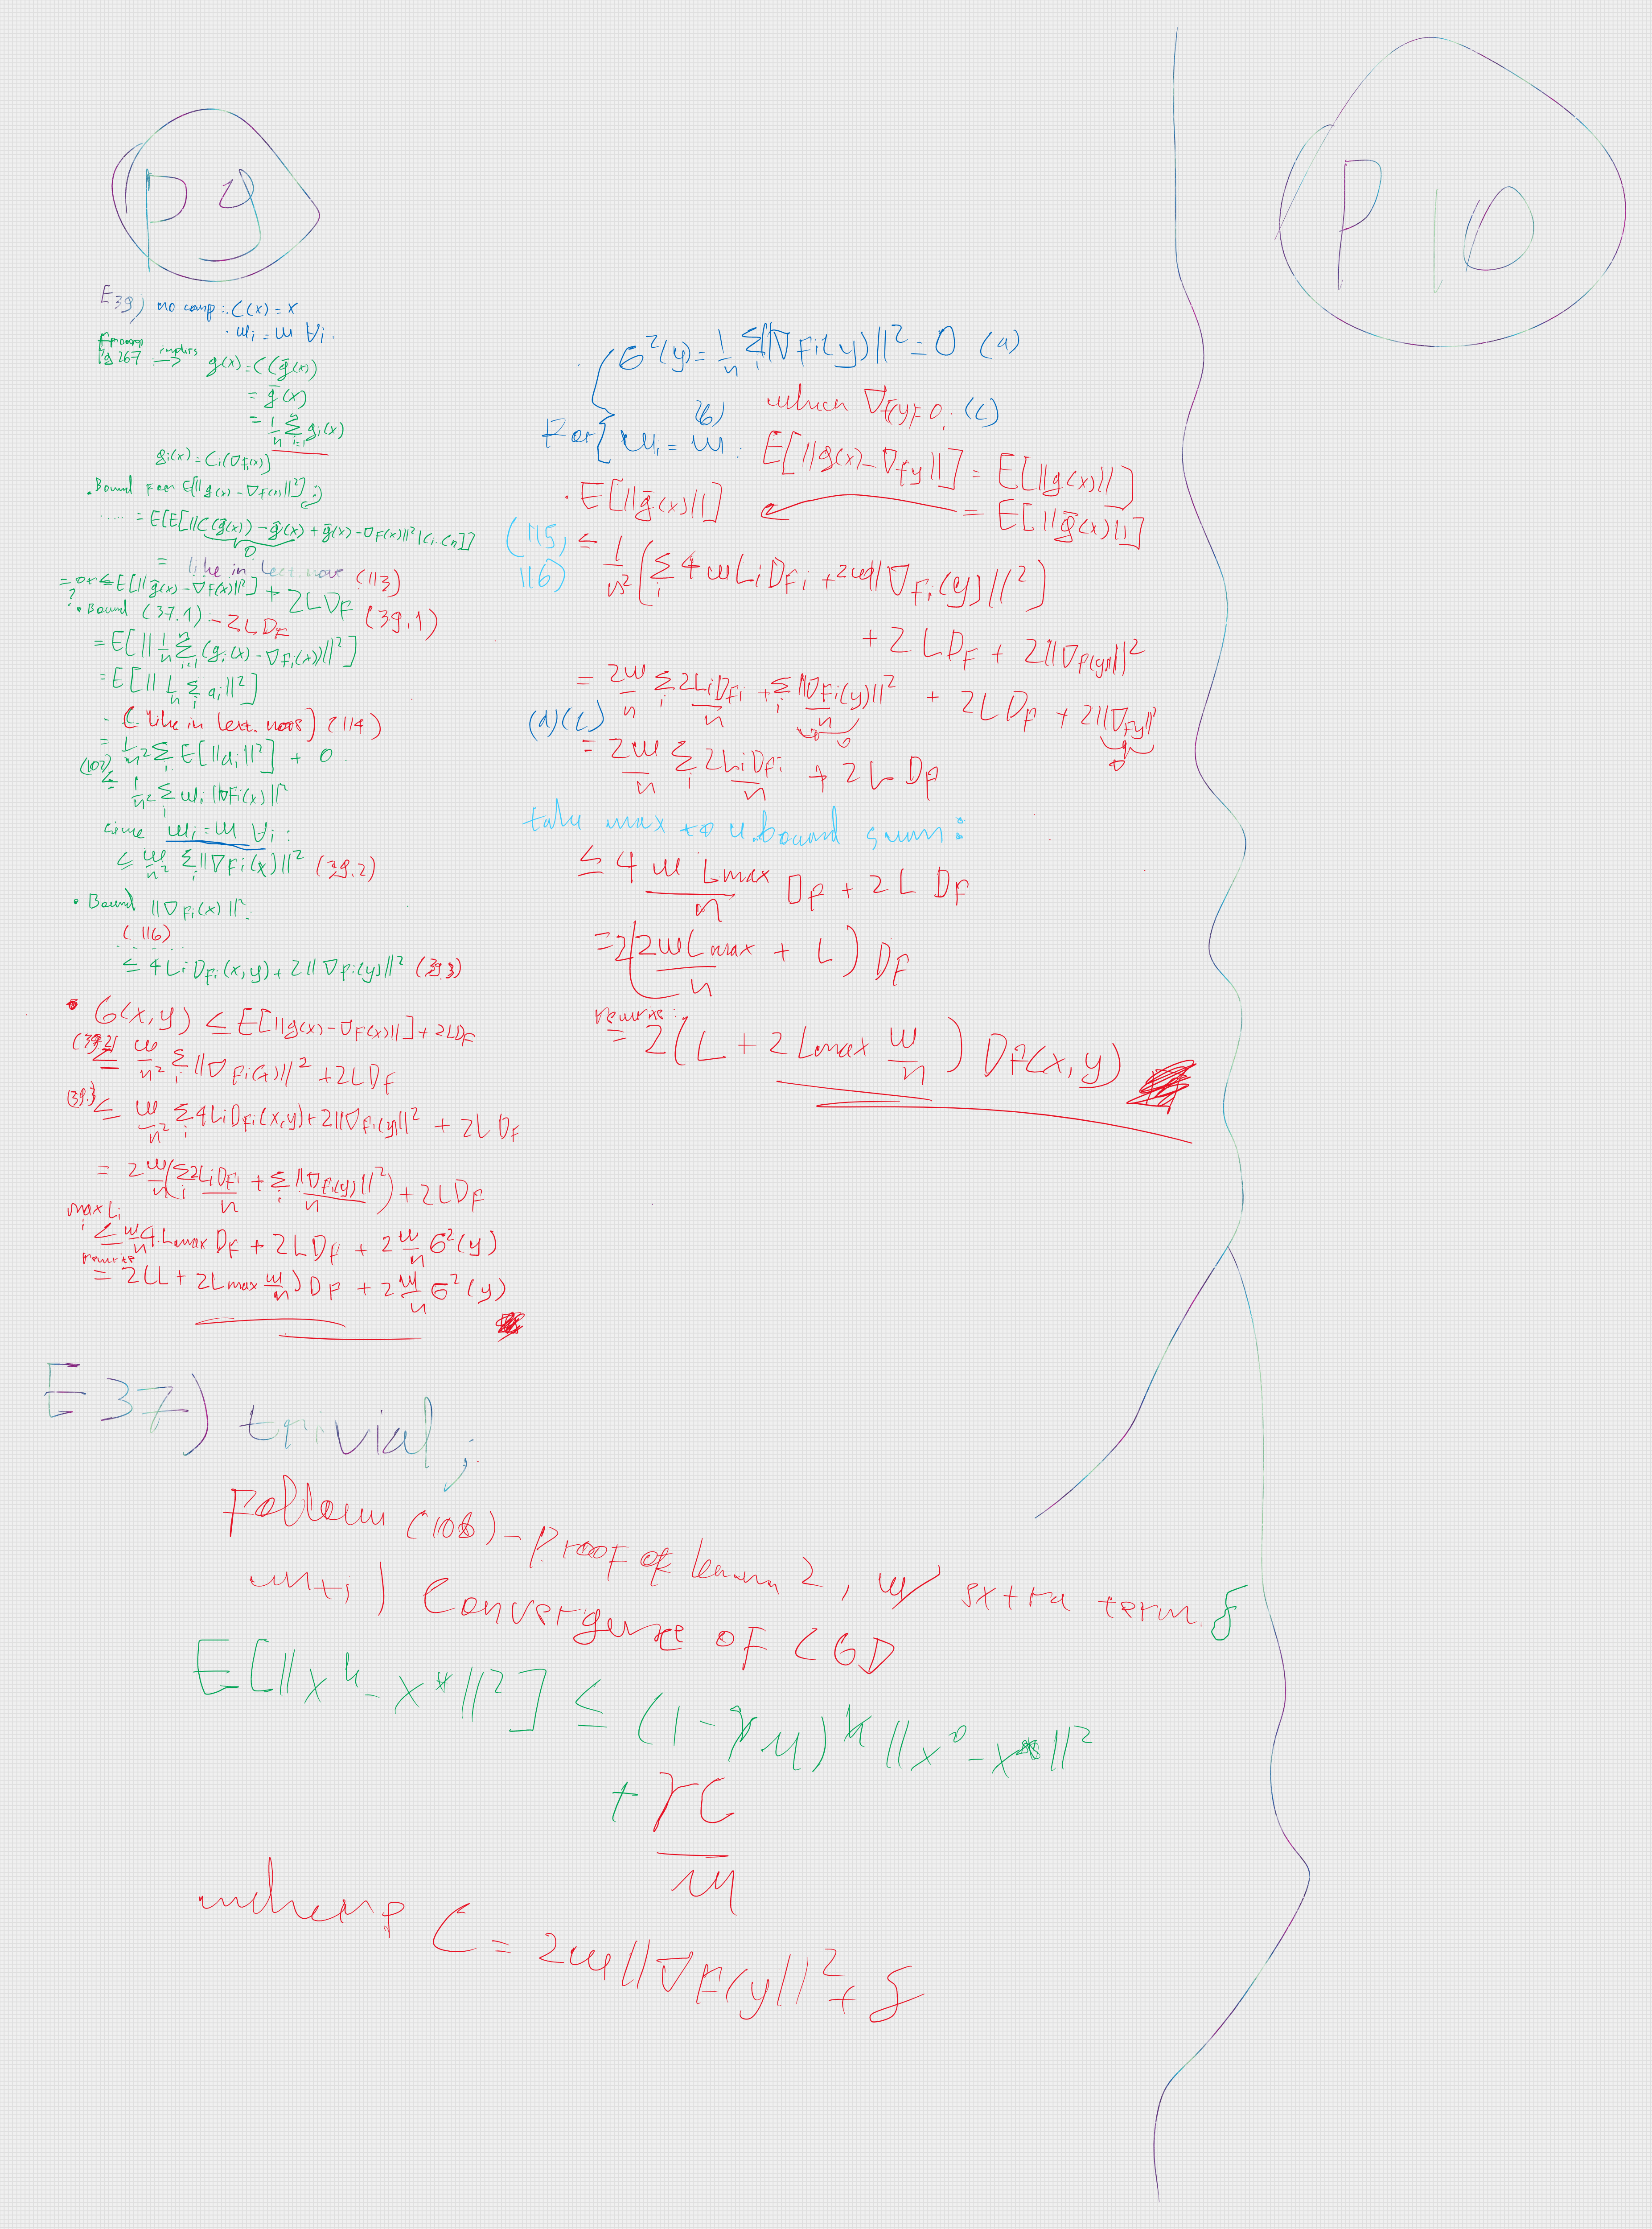
\includegraphics[width=\textwidth,height=\textheight,keepaspectratio]{img/P9.png}
\end{figure}

%\section*{Part 10}
% \subsection*{Exercise 41}
% \subsection*{Exercise 42}
(maybe) this is the other direction, if matrix is psd then E is psd: \hyperlink{https://math.stackexchange.com/questions/2650892/expectation-of-positive-semidefinite-random-matrix}{}

% \section*{Part 12}
% \subsection*{Exercise 55}
\hyperlink{https://arxiv.org/pdf/2206.10452.pdf}{}


\end{document}